\documentclass[11pt]{article}
\usepackage[utf8]{inputenc}
\usepackage[spanish]{babel}
\usepackage{amsmath}
\addto\captionsspanish{\renewcommand{\tablename}{Tabla}}
\usepackage{ifpdf}
\usepackage{array}
\usepackage[top=0.4in, bottom=1in, left=0.7in, right=0.7in]{geometry}
\newcolumntype{L}[1]{>{\raggedright\let\newline\\\arraybackslash\hspace{0pt}}m{#1}}
\newcolumntype{C}[1]{>{\centering\let\newline\\\arraybackslash\hspace{0pt}}m{#1}}
\newcolumntype{R}[1]{>{\raggedleft\let\newline\\\arraybackslash\hspace{0pt}}m{#1}}
\ifpdf
    \usepackage[pdftex]{graphicx}   % to include graphics
    \pdfcompresslevel=9 
    \usepackage[pdftex,     % sets up hyperref to use pdftex driver
            plainpages=false,   % allows page i and 1 to exist in the same document
            breaklinks=true,    % link texts can be broken at the end of line
            colorlinks=true,
            pdftitle=My Document
            pdfauthor=My Good Self
           ]{hyperref} 
    \usepackage{thumbpdf}
\else 
    \usepackage{graphicx}       % to include graphics
    \usepackage{hyperref}       % to simplify the use of \href
\fi


\title{Sistemas de Inteligencia Artificial\\
Redes Neuronales\\}
\author{Esteban Pintos (51048) - Cristian Pereyra (51190) - Matías De Santi (51051)}
\date{24 de Abril de 2013}

\begin{document}
\maketitle

\section{Introducción}
    \par En este informe se detalla la resolución del trabajo práctico número 2 de la materia. El mismo consistió en el desarrollo de una red neuronal multicapa con el estudio de diferentes funciones de activación para poder aproximar puntos desconocidos de una serie temporal.
\section{Desarrollo}
    \subsection{Modelado del problema}
   
    \par Se representó la red neuronal como una matriz con los pesos de todas las conexiones. Enumerando los nodos de izquierda a derecha comenzando por la capa de entrada es como se representan los pesos por fila en esta matriz.
    \par Además de los valores de la red, se mantuvo una  matriz de tres dimensiones. En la misma se puede encontrar por cada capa de la red las entradas o salidas de las neuronas según corresponda. En el primer valor del índice que itera por la dimensión que representa las capas, se encuentran las diferentes entradas de la red, es decir los patrones de entrenamiento. Luego por cada capa oculta se encuentran las salidas generadas por estas y finalmente para la capa de salida los valores que llegan a la misma que se transforman en el output de la red neuronal. Inicialmente a cada capa se le agrega el valor 1 como umbral. Esta matriz fue utilizada para entrenar la red.
    \par Modelar el problema de esta manera nos permitió calcular los valores generados en cada iteración simplemente iterando por la cantidad de capas y multiplicando las matrices mencionadas anteriomente (transponiendo la primera).
    \subsection{Elección de patrones}
    \par Para la elección de los patrones de entrenamiento se optó por tomar un subconjunto aleatorio del total dado un porcentaje que es parametro de la red. Por ejemplo, si se elige tomar un 70\% como patron de entrenamiento, el 30\% restante se toma como conjunto de testeo. Se decidió realizarlo de esta manera ya que se ajusta más a una situación real donde no se eligen los puntos de entrada, sino que se entrena a la red con los que se poseen en ese momento.
    \subsection{Funciones de activación}
    \par Para los casos de prueba llevados a cabo en la implementación de la red neural se utilizaron diferentes funciones de activación: La tangente hiperbólica \begin{eqnarray} \label{eq:solve} f(x) = tanh(x) \end{eqnarray} y la función exponencial \begin{eqnarray} \label{eq:solve} f(x) = \frac{2}{1+ e^{-\beta x}}-1 \end{eqnarray} 
    \par La función exponencial fue modificada para que la imagen caiga en los valores $y \in [-1 ,1]$.
    \subsection{Procesamiento de los patrones}
    \par Con el conjunto de patrones de entrenamiento ya elegidos, se realizan $n$ iteraciones sobre los mismos. En cada iteración se van eligiendo a los mismos de forma aleatoria y se calculan los valores de salida de la red neuronal y el error de la siguiente manera:
    \begin{eqnarray} \label{eq:solve} e = S_{i} - O_{i} \end{eqnarray} donde $S_{i}$ es el output esperado y $O_{i}$ es el output obtenido por la red neuronal para ese patrón dado. Luego se calculan los deltas realizando backpropagation y se corrigen los pesos de todas las conexiones. Al final de la iteración, luego de haber entrenado a la red con todos los patrones, se calcula el error cuadratico medio de la siguiente manera:
    \begin{eqnarray} \label{eq:solve} \sum\limits_{i=0}^N \frac{{(S_{i} - O_{i})}^2}{N} \end{eqnarray} donde N es la cantidad de patrones totales. Cuando el error medio es menor a un valor ingresado por parametro, se da por finalizado el aprendizaje de la red neuronal.
    
    \subsection{Mejoras implementadas}
    \par Debido que al correr la red neuronal con los parámetros de la función temporal, la misma luego de varias iteraciones tendía a estancarse en un mínimo local decidimos implementar diferentes funciones para evitar esto.
    \subsubsection{Variación backpropagation}
    \par Se decidió modificar el calculo de la Regla Delta de la siguiente manera \begin{eqnarray} \label{eq:solve} \delta_{i}^{\mu} = [g'(h_{i}^{\mu})+0.1]*e \end{eqnarray} de esta manera se puede llegar a evitar minimos locales debido a que la derivada de la función vale 0 en aquellos puntos que son mínimos locales.
    \subsubsection{Momentum}
    \par Para darle peso a bifurcaciones que pueden llegar al correcto aprendizaje de la red se decidió implementar el momentum de la siguiente manera: \begin{eqnarray} \label{eq:solve} w(t+1) = -\frac{\partial E}{\partial w_{ij}} + \alpha w(t) \end{eqnarray}
    \subsubsection{Eta adaptativo}
    \par Debido a que un eta constante puede ser bueno en algunos momento del aprendizaje de la red y en otros no. Si el error no disminuye en una cantidad de iteraciones entonces este debe ser decrementado, en caso contrario debe ser incrementado. El incremento se realiza con un valor de $1.2$ y el decrecimiento se realiza bajando su valor en un 90\%.
    \subsection{Arquitecturas}
    \par La elección de una correcta arquitectura para la red neuronal es sumamente importante para lograr un correcto aprendizaje. Elegir una arquitectura no apropidada para el problema a resolver podría generar que la red no aprenda nunca aunque se la deje correr durante $n$ iteraciones.
    \par Se intentó entrenar la red con una sóla neurona en la capa oculta. Como era de esperarse, esta red no fue útil ya que no logró aprender el conjunto de entrenamiento y mucho menos el conjunto de testeo.
    \par Luego se fueron probando diferentes arquitecturas. El objetivo en un principio era encontrar arquitecturas que aprendieran el conjunto de entrenamiento y pudieran generalizar de manera aceptable el conjunto de testeo. Luego de probar diferentes arquitecturas (arquitecturas con más de una capa, con más y menos neuronas) decidimos que estas eran las más significativas para evaluar:
        \begin{itemize}
            \item dos capas: una con 9 y otra con 6 neuronas.
            \item una sóla capa con 20 neuronas.
            \item dos capas: una con 5 y otra con 4 neuronas.
            \item dos capas: una con 3 y otra con 2 neuronas.
        \end{itemize}
\section{Resultados y análisis}
    \subsection{Efecto del momentum}
    \par Si bien el desarrollo de la red neuronal no es complejo, la mayor complejidad se nos presentó a la hora de elegir los parámetros de la red. Una variación en alguno de los ellos hace que la misma se comporte de maneras totalmente distintas y arroje resutados no deseados.
    \par En nuestro caso en particular, la primera implementación de momentum utilizaba \begin{math}\alpha\end{math} igual a 0.9. Al correr la red con esta configuración, el error cuadrático medio del conjunto de entrenamiento era siempre superior a 0.2. Al pasar el conjunto de testeo, el error cuadrático medio era cercano a 1, con un error máximo de 3.572. Sin embargo, al bajar \begin{math}\alpha\end{math} a 0.1, la red se comportó de otra manera y logró un error cuadrático medio del conjunto de entrenamiento por debajo de 0.05. El error cuadrático medio del conjunto de testeo bajó a valores cercanos a 0,06 con un error máximo de 0.672.
    Es altamente probable que la superficie sobre la cual se están explorando las soluciones tenga pocos cambios. De esta manera, si se tiene un valor de \begin{math}\alpha\end{math} elevado, ante pequeños cambios la red reacciona bruscamente. Por otro lado, cuando alpha toma valores bajos (alrededor de 0.1), la reacción frente a cambios en la superficie es más suave y permite que la exploración continue en la dirección correcta.
    \par Otra reacción que se pudo observar al aumentar el valor de \begin{math}\alpha\end{math} fue que el valor de los pesos de las conexiones entre neuronas era elevado y por lo tanto las neuronas de las capas ocultas saturaban rápidamente. De esta manera, el aprendizaje de la red se ve impedido. Al disminuir el valor de \begin{math}\alpha\end{math}, los pesos de las conexiones no aumentaban de la misma manera, la red no saturaba y por lo tanto el aprendizaje era mejor.
    \subsection{Funciones de Activación}
    \par Dado que la función de activación sigmoidea exponencial es igual a \begin{math} tanh(\frac{x}{2})\end{math}, utilizar una u otra función es indistinto. Para que la exponencial se comporte como la hiperbólica es necesario cambiar el $\beta$ utilizado y ambas funciones se comportan idénticamente.
    \subsection{Arquitecturas}
    \par Realizamos distintas pruebas sobre las arquitecturas mencionadas con el fin de definir cuál de las dos daba mejores resultados. Se variaron los tamaños de los conjuntos de prueba, se probaron sin momentum y sin eta adaptativo y se los probó con 2 y 3 puntos de entrada para poder estimar el siguiente.
    \par La tabla \ref{table:Comparacion1} muestra una comparación entre las arquitecturas con una entrada de 2 puntos, con un conjunto de entrenamiento de 800 sets, eta adaptativo y momentum activado.
        \begin{table}[htdp] 
        \begin{center}
        \begin{tabular}{|C{2cm}|C{2cm}|C{1cm}|C{1cm}|C{2cm}|C{2cm}|C{2cm}|C{2cm}|}
            \hline Arquitectura & Tamaño del training set & Eta variable & Momentum & E.C.M. del cjto de entrenamiento & E.C.M. del cjto de testing & Error máximo en test & Error mínimo en test \\ \hline\hline
            2 9 6 1 & 800 & Si & Si	& 0.0059784 & 0.0776 & 0.81839 & 0.00077428\\ \hline
            2 20 1 & 800 & Si & Si & 0.007384 & 0.11201 & 1.1538 & 0.0031247\\ \hline
            2 5 4 1 & 800 & Si & Si & 0.03458 & 0.50746 & 3.1451 & 0.0010729\\ \hline
            2 3 2 1 & 800 & Si & Si & 0.14684 & 1.9140 & 5.7589 & 0.0049337\\ \hline
        \end{tabular}
        \end{center}
        \caption{Comparación de arquitecturas}
        \label{table:Comparacion1}
        \end{table}
        
        \begin{figure}[htbp]
    		\centering
				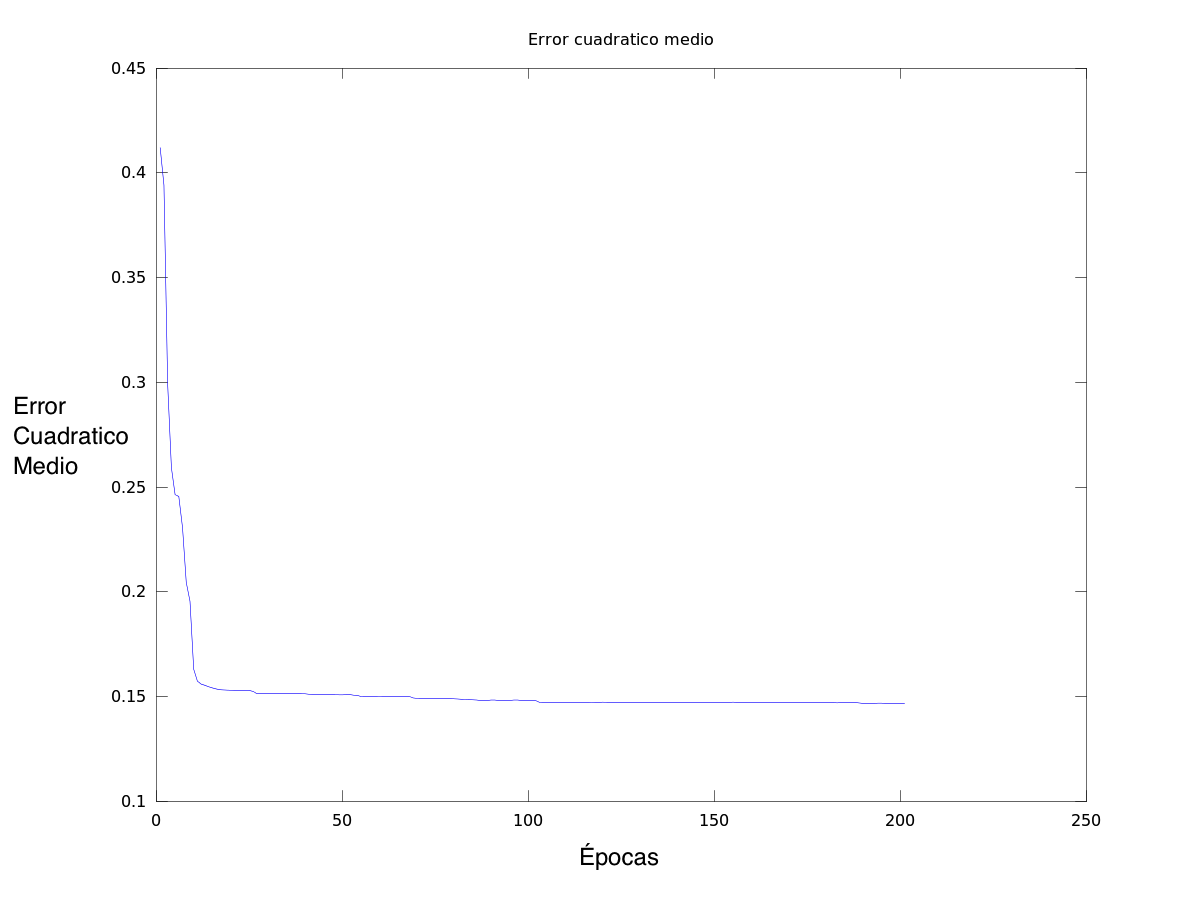
\includegraphics[width=1.0\textwidth]{img/3-2-1/ecm.png}
			\caption{Error cuadrático medio para un una arquitectura 2-3-2-1}
			\label{fig:321}
		\end{figure}
        
        \begin{figure}[htbp]
        	\centering
				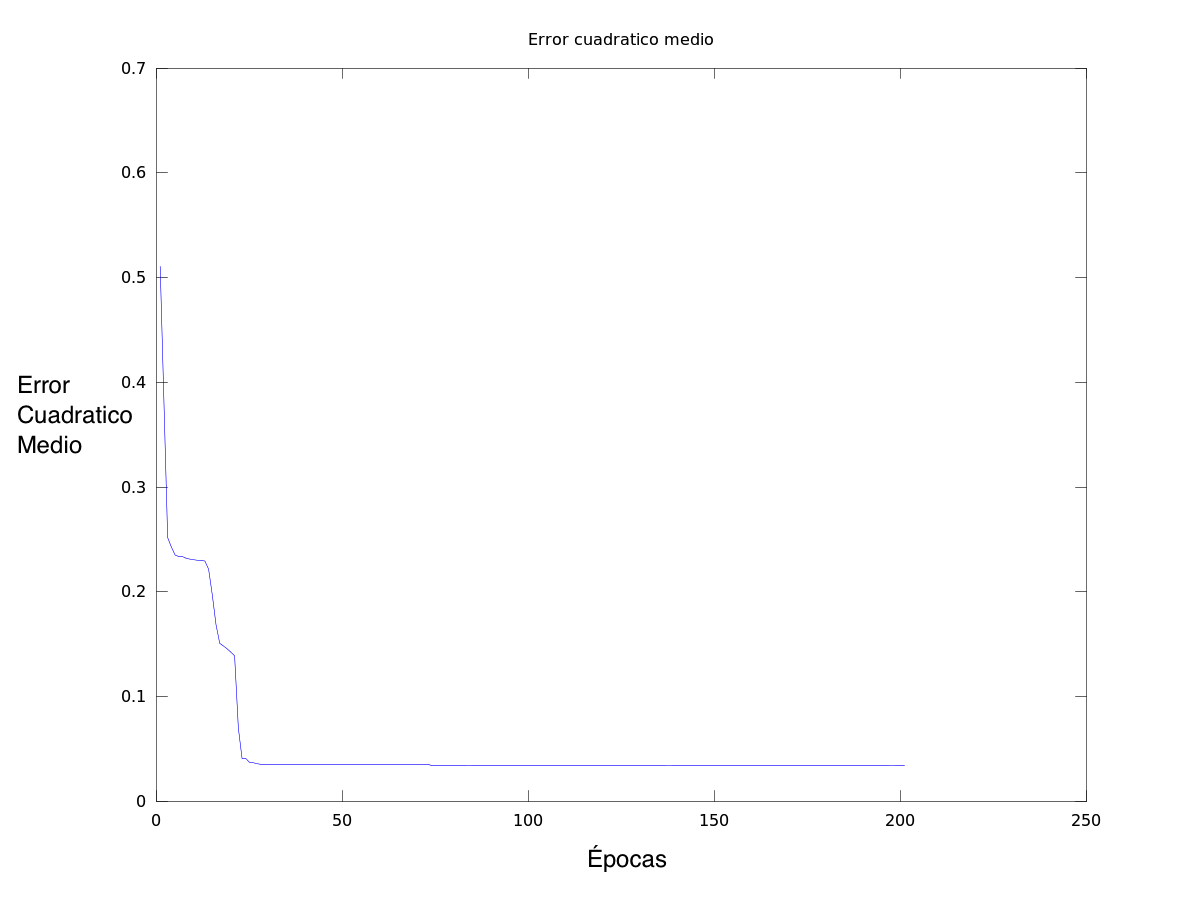
\includegraphics[width=1.0\textwidth]{img/5-4-1/ecm.png}
			\caption{Error cuadrático medio para un una arquitectura 2-5-4-1}
			\label{fig:541}
		\end{figure}
        
        \begin{figure}[htbp]
            \centering
				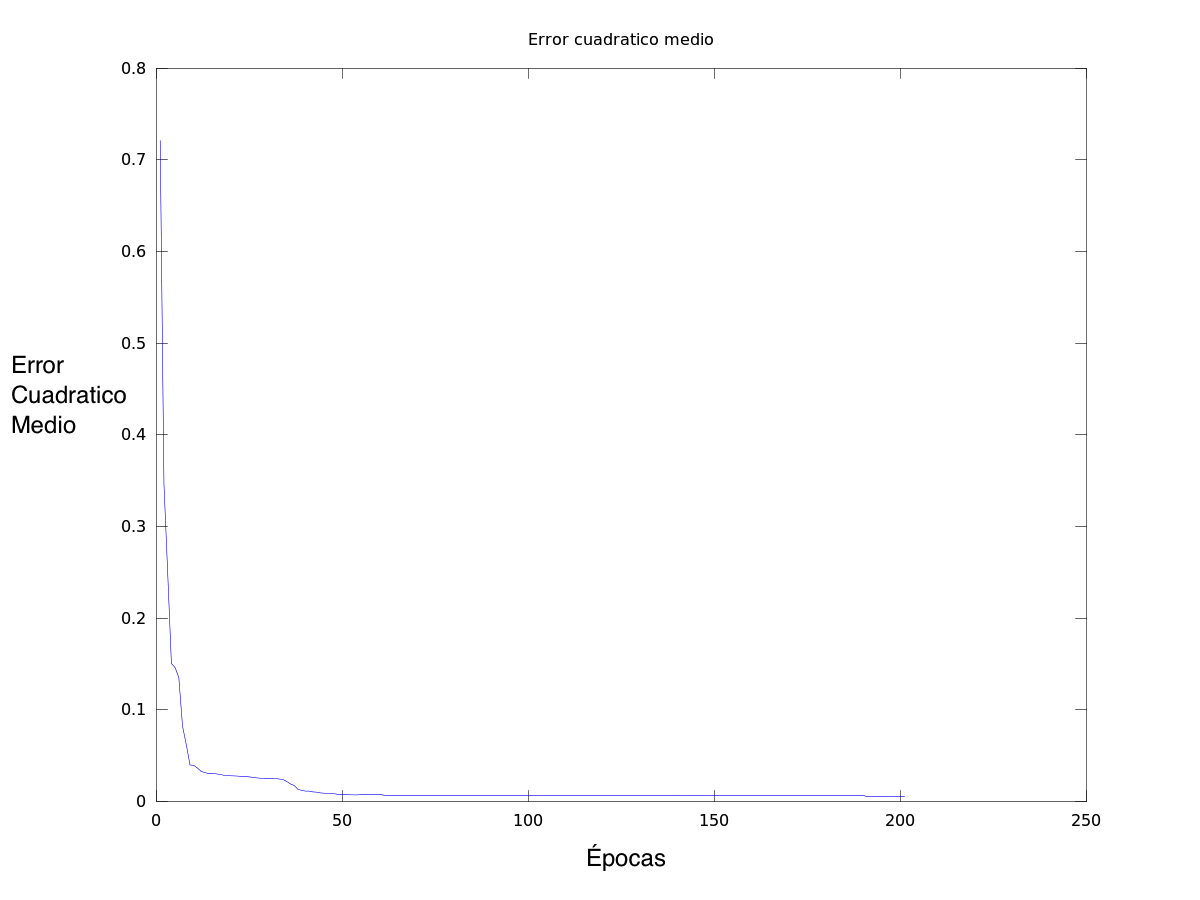
\includegraphics[width=1.0\textwidth]{img/9-6-1/ecm.png}
			\caption{Error cuadrático medio para un una arquitectura 2-9-6-1}
			\label{fig:961}
		\end{figure}
        
        \begin{figure}[htbp]
            \centering
    			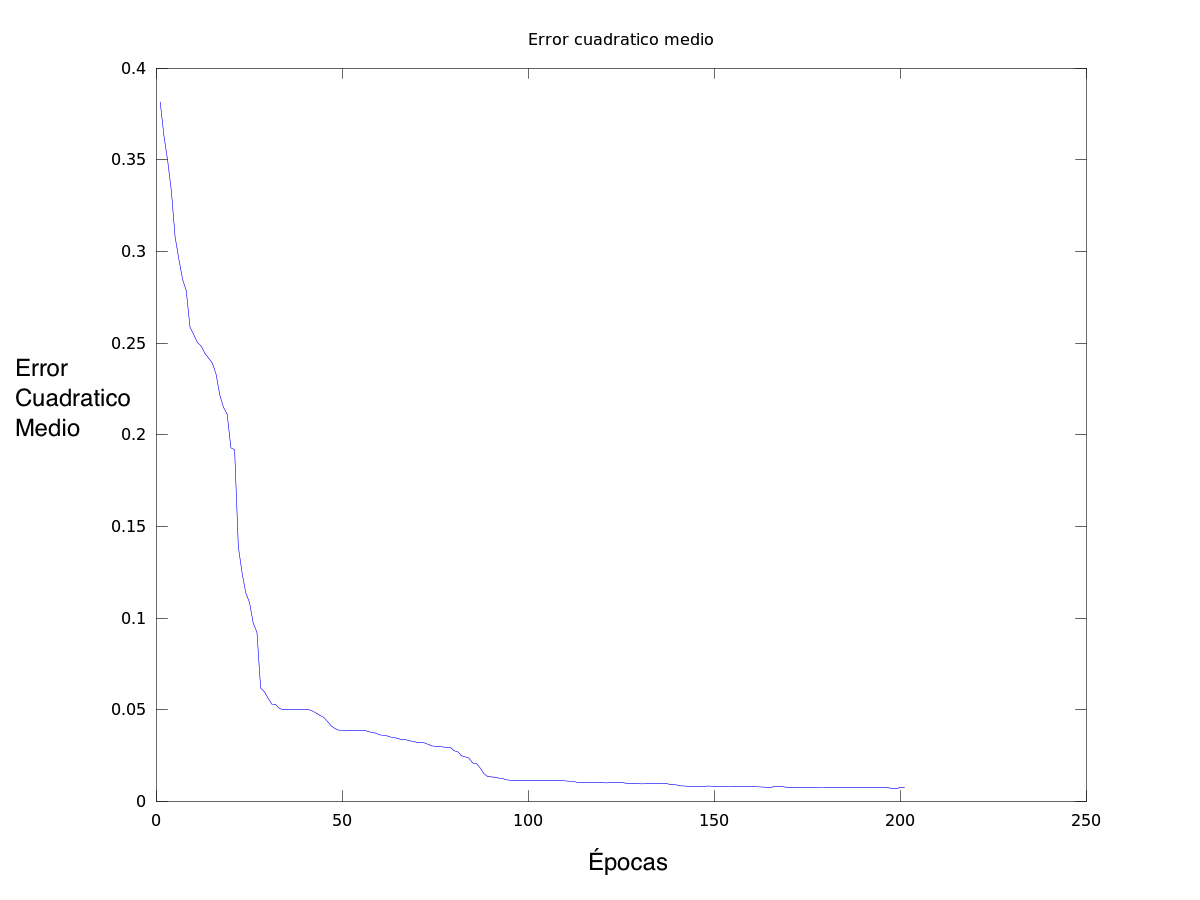
\includegraphics[width=1.0\textwidth]{img/20-1/ecm.png}
			\caption{Error cuadrático medio para un una arquitectura 2-20-1}
			\label{fig:201}
		\end{figure}
        
        \begin{figure}[htbp]
            \centering
        		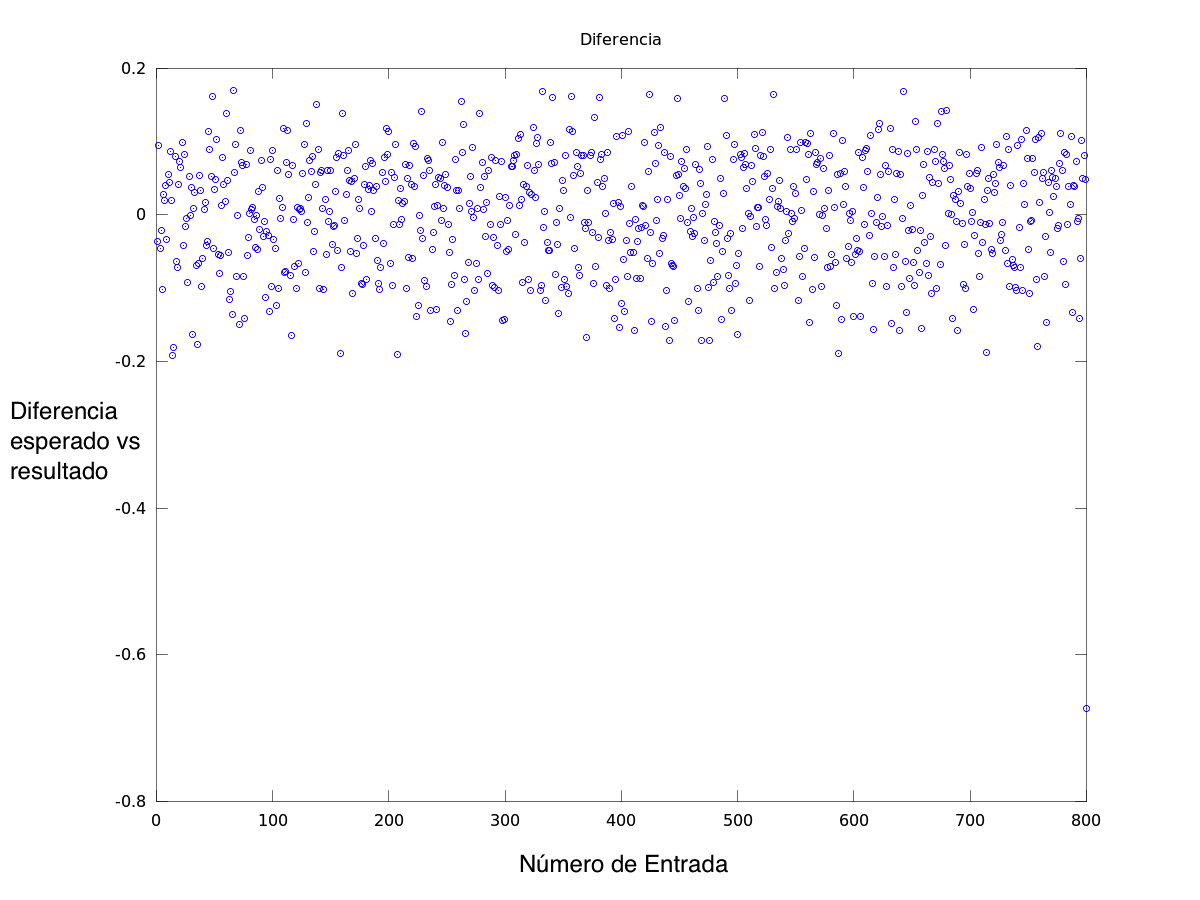
\includegraphics[width=1.0\textwidth]{img/9-6-1/diferencia_final.png}
			\caption{Diferencia puntual de estesperado/resultado con la mejor arquitectura (9-6-1)}
			\label{fig:961diff}
		\end{figure}
        
    \par Observando los primeros dos de la tabla, se puede ver que la arquitectura de 2 capas ocultas tuvo un error cuadrático medio en el conjunto de entrenamiento y en el de testeo ligeramente menor a la arquitectura de una capa oculta. Sin embargo, la mayor diferencia puede apreciarse en el máximo error obtenido en el conjunto de testing. En cuanto a la arquitectura de dos capas ocultas, obtuvo un error máximo de 0.82 mientras que la de 1 sóla capa obtuvo 1.15.
    \par Siguiendo con las configuraciones anteriores, la red con 2 capas ocultas logró categorizar un 85\% de los puntos del conjunto de testeo con un error menor que 0.4, mientras que la otra red logró categorizar un 83\% de los datos.
    \par En términos generales, se puede ver que las últimas dos arquitecturas de la tabla empiezan a denotar un error mayor, esto es debido a que la arquitectura no tiene la suficiente cantidad de neuronas para poder aproximar correctamente el problema. También puede verse que con un aumento de menos del doble de neuronas se pueden obtener resultados varias veces mejores respecto a una configuración con menos neuronas.
    \par Finalmente se pueden ver los gráficos \ref{fig:321}, \ref{fig:541}, \ref{fig:961}, \ref{fig:201} en los cuales se ve cómo progresa el error cuadrático medio en cada arquitectura. Por otro lado, la figura \ref{fig:961diff} muestra gráficamente el error lineal de cada punto evaluado en el conjunto de entrenamiento 2-9-6-1.
    \section{Conclusiones}
    \par Luego de haber desarrollado este trabajo práctico y de haber probado la red neuronal bajo diferentes situaciones, podemos concluir que los parámetros (\begin{math}\alpha\end{math}, \begin{math}\beta\end{math}, etc) son sumamente importantes para el correcto funcionamiento de la red. Un pequeño cambio en cualquiera de ellos puede hacer que la red aprenda y obtenga resultados con un error cuadrático medio bajo o que aprenda pero con un error alto.
    \par Por otra parte, las arquitecturas juegan un rol importante también ya que no cualquier arquitectura es adecuada al problema. Una red con una gran cantidad de neuronas en la capa oculta va a aprender el problema, pero probablemente no generalice bien ya que aprende de memoria. Por otra parte, utilizar pocas neuronas puede significar que la red directamente no aprenda. La segunda situación claramente no es deseable, mientras que la segunda depende del problema. En nuestro caso, el poder de generalización de la red era muy importante.
      
\clearpage
\onecolumn
\appendix
\end{document}
